\documentclass[11pt]{article}
\usepackage[margin=1in]{geometry}
\usepackage{amsmath, amssymb, amsthm, esint}
\usepackage{fancyhdr}
\usepackage{tikz, tikz-3dplot}
% \usepackage{hyperref}
\usepackage{enumitem}
\usepackage{float}
\usepackage{booktabs}
\usepackage{array}
\usepackage{cancel}
\usetikzlibrary{decorations.pathreplacing}

\setlength{\headheight}{14pt}
\fancyhf{}
\lhead{Complex Analysis}
\cfoot{\thepage}

\begin{document}
\pagestyle{plain}
\begin{center}
    \tableofcontents
\end{center}
\newpage
\setcounter{page}{1}
\pagestyle{fancy}
\section{Complex Number and the Complex Plane}
\subsection{Complex Numbers and Their Properties}
We define \textbf{the imaginary unit} $i$ by $i^2 = -1$. A \textbf{complex number} is any number of the form 
\[
    z = a + ib,\quad a, b\in\mathbb{R}
\]
where $a$ is real part of $z$, and $b$ is the imaginary part. That is,
\[
    \text{Re}(z) = a, \text{Im}(z) = b
\]
In addition, $z_1 = z_2$ are equal if $a_1 = a_2,\,b_1 = b_2$.
\subsubsection*{Arithmetic Operations}
let $z_1 = a_1 + b_1i,\,z_2 = a_2 + b_2i$
\begin{itemize}
    \item Addition: $z_1 + z_2 = (a_1+a_2)+ (b_1+b_2)i$
    \item Subtraction: $z_1 - z_2 = (a_1-a_2)+ (b_1-b_2)i$
    \item Multiplication: $z_1 z_2 = (a_1 + b_1i)(a_2 + b_2i) = a_1a_2 + (a_1b_2 + a_2b_1)i - b_1b_2$
    \item Division: $\displaystyle\frac{z_1}{z_2} = \frac{a_1 + b_1i}{a_2 + b_2i} = \frac{a_1a_2 + b_1b_2}{a_2^2+b_2^2} + \frac{a_2b_1-a_1b_2}{a_2^2+b_2^2}i$
\end{itemize}
The commutitive, associative, and distributive laws also hold for complex numbers:
\begin{itemize}
    \item Commutitive laws: $\begin{cases}z_1+z_2 = z_2+z_1\\ z_1z_2 = z_2z_1\end{cases}$
    \item Associative laws: $\begin{cases}z_1+(z_2+z_3) = (z_1+z_2)+z_3\\ z_1(z_2z_3) = (z_1z_2)z_3\end{cases}$
    \item Distributive law: $z_1(z_2+z_3) = z_1z_2 + z_1z_3$
\end{itemize}
\subsubsection*{Complex Conjugate}
The \textbf{complex conjugate} of $z$, denoted by $\overline{z}$ or $z^\ast$, is obtained by changing the sign of its imaginary part:
\[
    \overline{z} = z^\ast = a - bi.
\]
The complex conjugate satisfies the following properties:
\begin{itemize}
    \item $\displaystyle \overline{z_1 \pm z_2} = \overline{z_1} \pm \overline{z_2}$
    \item $\displaystyle \overline{z_1 z_2} = \overline{z_1} \, \overline{z_2}$
    \item $\displaystyle \overline{\left(\frac{z_1}{z_2}\right)} = \frac{\overline{z_1}}{\overline{z_2}}, \quad (z_2 \neq 0)$
\end{itemize}
\subsection{Complex Plane}
A complex number $z = a + bi$ can be uniquely represented by an ordered pair of real numbers $(a, b)$.  
In this way, we associate each complex number with a point in the coordinate plane, or equivalently,  
with the position vector $\vec{z} = \langle a, b \rangle$ originating from the origin.
\begin{center}
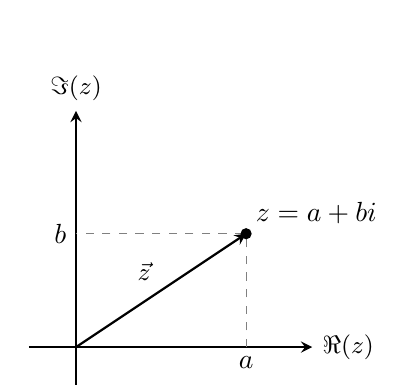
\begin{tikzpicture}[scale=1.2, >=stealth]
    \draw[->, thick] (-0.5,0) -- (2.5,0) node[right] {\small $\Re(z)$};
    \draw[->, thick] (0,-0.5) -- (0,2.5) node[above] {\small $\Im(z)$};
    
    \draw[->, thick] (0,0) -- (1.8,1.2) node[midway, above left] {\small $\vec{z}$};
    
    \draw[dashed, gray] (1.8,0) -- (1.8,1.2) -- (0,1.2);
    
    \filldraw[black] (1.8,1.2) circle (1.5pt) node[above right] {$z = a + bi$};
    \node[below] at (1.8,0) {$a$};
    \node[left] at (0,1.2) {$b$};
\end{tikzpicture}
\end{center}
The \textbf{modulus} (or \textbf{absolute value}) of a complex number is the length of its vector representation:
\[
    |z| = \sqrt{a^2 + b^2} = \sqrt{z\,\overline{z}}.
\]
Thus, each complex number corresponds both to a point $(a, b)$ in the plane and to a vector $\vec{z}$ from the origin to that point.
\subsubsection*{The difference between two complex number}
The difference between two complex numbers $z_2 - z_1$ represents the vector pointing from $z_1$ to $z_2$:
\begin{center}
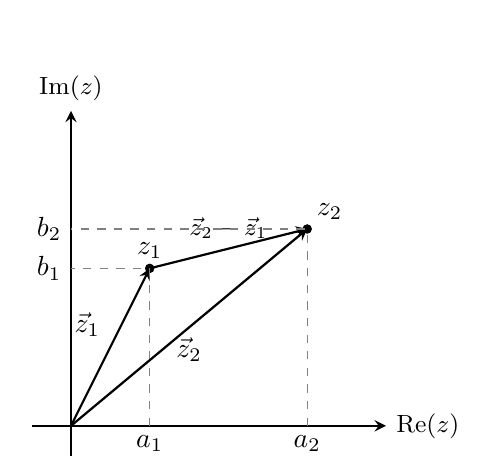
\begin{tikzpicture}[scale=1, >=stealth]
    \draw[->, thick] (-0.5,0) -- (4,0) node[right] {\small Re($z$)};
    \draw[->, thick] (0,-0.5) -- (0,4) node[above] {\small Im($z$)};
    
    \filldraw[black] (1,2) circle (1.5pt) node[above] {$z_1$};
    \filldraw[black] (3,2.5) circle (1.5pt) node[above right] {$z_2$};
    
    \draw[->, thick] (0,0) -- (1,2) node[midway, above left] {$\vec{z}_1$};
    \draw[->, thick] (0,0) -- (3,2.5) node[midway, below] {$\vec{z}_2$};
    
    \draw[->, thick] (1,2) -- (3,2.5) node[midway, above] {\small $\vec{z}_2 - \vec{z}_1$};
    
    \draw[dashed, gray] (3,0) -- (3,2.5) -- (0,2.5);
    \draw[dashed, gray] (1,0) -- (1,2) -- (0,2);
    
    \node[below] at (1,0) {$a_1$};
    \node[left] at (0,2) {$b_1$};
    \node[below] at (3,0) {$a_2$};
    \node[left] at (0,2.5) {$b_2$};
\end{tikzpicture}
\end{center}
\subsubsection*{Inequalities}
\subsection{Polar Representation of Complex Numbers}
Complex numbers can also be represented in terms of polar coordinatess. 
\begin{center}
    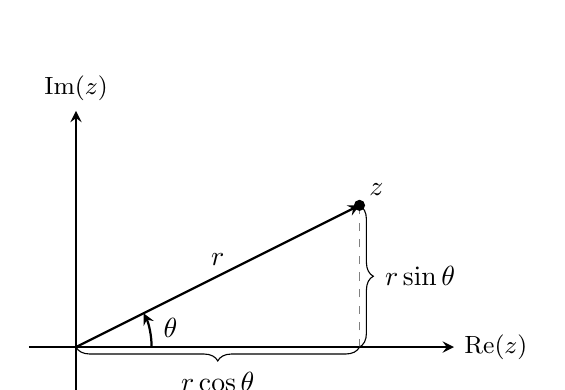
\begin{tikzpicture}[scale=1.2, >=stealth]
        \draw[->, thick] (-0.5,0) -- (4,0) node[right] {\small Re($z$)};
        \draw[->, thick] (0,-0.5) -- (0,2.5) node[above] {\small Im($z$)};
        
        \draw[->, thick] (0,0) -- (3,1.5)node[midway, above] {$r$};

        \draw[dashed, gray] (3,0) -- (3,1.5) ;

        \filldraw[black] (3,1.5) circle (1.5pt) node[above right] {$z$};

        \draw[decorate,decoration={brace, amplitude=5pt, mirror}] (0,0) -- (3,0) 
            node[midway, below, yshift=-2mm] {$r\cos\theta$};
        \draw[decorate,decoration={brace, amplitude=5pt, mirror}] (3,0) -- (3,1.5) 
            node[midway, right, xshift=2mm] {$r\sin\theta$};

        \draw[thick, ->] (0.8,0) arc[start angle=0, end angle=26.565, radius=0.8cm];
        \node at (1,0.2) {$\theta$};
    \end{tikzpicture}
\end{center}
This is called the \textbf{polar form} of a complex number:
\[
    z = r(\cos\theta + i\sin\theta)
\]
where $r = \sqrt{a^2 + b^2}$ and $\theta = \text{arg}(z)$, called the argument of $z$
\subsubsection*{Principle Argument}
$\theta$ is called the \textbf{principle value} or \textbf{principle argument} of $z$, denoted by Arg($z$), if
\[
    -\pi < \theta \leq \pi
\]
In general, arg($z$) and Arg($z$) are related by
\[
    \text{arg}(z) = \text{Arg}(z) + 2n\pi, \quad n = 0,\,\pm 1,\,\pm 2,\,\dots 
\]

\end{document}